\section{CMOS MAPS}

    %%%%%%%%%%%%%%%%%%%%%%%%%%%%%%%%%%%%%%%%
    %%  Slide 2: <CMOS MAPS concept>  %%
    %%%%%%%%%%%%%%%%%%%%%%%%%%%%%%%%%%%%%%%%
    \begin{frame}
        \frametitle{CMOS Monolitich Active Pixel Sensors}
        %forse anche la terza parentesi con minore circa 100 um
        \begin{columns}
            \column{0.4\textwidth}
                \vspace*{-0.6cm}
                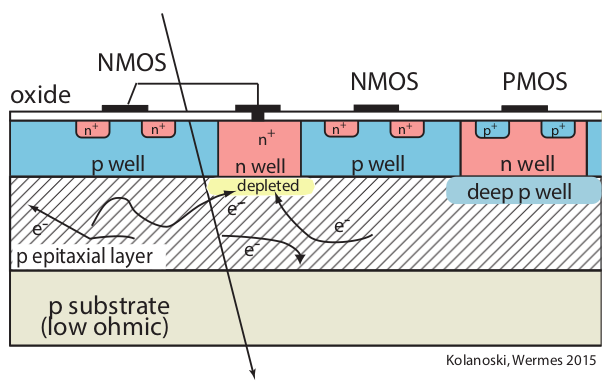
\includegraphics[width=1.15\linewidth]{figures/Pixel_detectors/MAPS_scheme.png}
            \column{0.6\textwidth}  
                \begin{tikzpicture}[overlay]
                    \draw[decorate,decoration={brace}]
                        (0,-0.6) -- node[xshift=2pt,anchor=west] {$\lesssim$\SI{5}{\um} electronics}(0,-1.15);
                \medskip
                    \draw[decorate,decoration={brace}]
                        (0,-1.25) -- node[xshift=2pt,anchor=west] {$\lesssim$\SI{50}{\um} sensor}(0,-1.9);
                \end{tikzpicture}
                \bigskip
                \begin{equation*}
                    \hspace{80pt} d \propto \sqrt{\rho V}
                \end{equation*}   
                \begin{equation*}
                    %\hspace{75pt} ENC^2 \propto \frac{4}{3} \frac{kT}{g_m} \frac{C_D ^2}{\tau_{sh}}
                    \hspace{80pt} ENC^2 \propto C_D ^2
                \end{equation*}  
                \begin{equation*}
                    %\hspace{75pt} \tau \propto \frac{1}{g_m}\frac{C_D}{C_f}
                    \hspace{80pt} \tau \propto C_D
                \end{equation*}  
                \begin{equation*}
                    \hspace{80pt} Q_{MIP}\propto d \sim 80 e^-/\si{\um}
                \end{equation*}  
            \end{columns}   
        \medskip 
        FORMAZIONE DEL SEGNALE
    \end{frame} 

    %%%%%%%%%%%%%%%%%%%%%%%%%%%%%%%%%%%%%%%%
    %%  Slide 2: <CMOS MAPS concept>  %%
    %%%%%%%%%%%%%%%%%%%%%%%%%%%%%%%%%%%%%%%%
    \begin{frame}
        \frametitle{CMOS Monolitich Active Pixel Sensors}
        %forse anche la terza parentesi con minore circa 100 um
        \begin{columns}
            \column{0.4\textwidth}
                \vspace*{-0.6cm}
                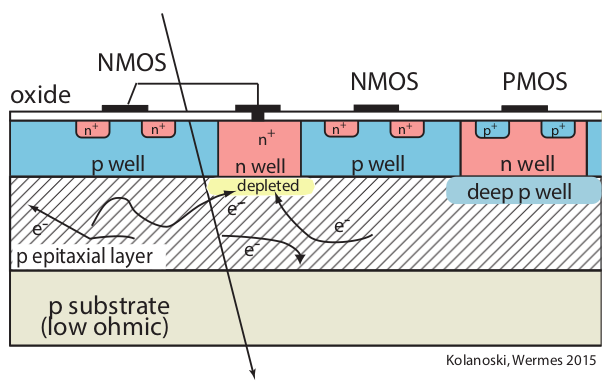
\includegraphics[width=1.15\linewidth]{figures/Pixel_detectors/MAPS_scheme.png}
            \column{0.6\textwidth}  
                \begin{tikzpicture}[overlay]
                    \draw[decorate,decoration={brace}]
                        (0,-0.6) -- node[xshift=2pt,anchor=west] {$\lesssim$\SI{5}{\um} electronics}(0,-1.15);
                \medskip
                    \draw[decorate,decoration={brace}]
                        (0,-1.25) -- node[xshift=2pt,anchor=west] {$\lesssim$\SI{50}{\um} sensor}(0,-1.9);
                \end{tikzpicture}
                \bigskip
                \begin{equation*}
                    \hspace{80pt} d \propto \sqrt{\rho V}
                \end{equation*}   
                \begin{equation*}
                    %\hspace{75pt} ENC^2 \propto \frac{4}{3} \frac{kT}{g_m} \frac{C_D ^2}{\tau_{sh}}
                    \hspace{80pt} ENC^2 \propto C_D ^2
                \end{equation*}  
                \begin{equation*}
                    %\hspace{75pt} \tau \propto \frac{1}{g_m}\frac{C_D}{C_f}
                    \hspace{80pt} \tau \propto C_D
                \end{equation*}  
                \begin{equation*}
                    \hspace{80pt} Q_{MIP}\propto d \sim 80 e^-/\si{\um}
                \end{equation*}  
            \end{columns}   
        \medskip 
        \begin{itemize}
            \item An epitaxial layer with doping few order of magnitude smaller than the subtrate is introduced below the surface
            \item Electronics is low resistivity while sensor needs high $\rho$, special technologies for the sensor have been implemented. 
            \item High resistivity allows for depleted epi-layer DMAPS
            \item If not completed depleted charge is collected by diffusion
            \item MAPS have a very low capacity 
        \end{itemize}
    \end{frame} 


    %%%%%%%%%%%%%%%%%%%%%%%%%%%%%%%%%%%%%%%%
    %%  Slide 1: <READOUT>  %%
    %%%%%%%%%%%%%%%%%%%%%%%%%%%%%%%%%%%%%%%%
    \begin{frame}
        \frametitle{Front end}
        RIFAI CON LA TABELLINA COME DICEVA FORTI SEGNANDO LE COSE PER MONOPIX1
            \begin{columns}
                \column{0.7\textwidth}  
                \textbf{Pixel area economy} and dimension of components are extremely relevant. \\
                MAPS usage allowed by miniaturization of components: starting from \SI{600}{nm} down to 120-180{nm} CMOS process.
                \column{0.4\textwidth}  
                    \begin{figure}[h!]
                        \vspace*{-0.85cm}
                        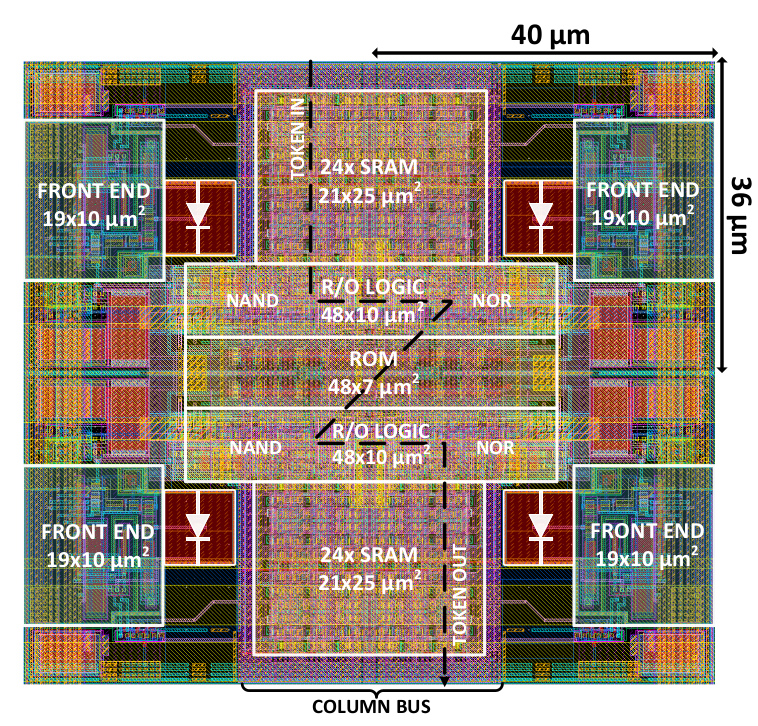
\includegraphics[width=1.05\linewidth]{figures/Monopix1/Monopix1_2x2pixelsgroup.png}
                    \end{figure}
            \end{columns}
        \begin{itemize}
            \item Analog or digital output
            \item Triggered or triggerless
            \item Buffer on pixel to store more than one hit data
            \item Rolling shut or sparsified (data push) readout, for example column drain is one of the most popular.
        \end{itemize}
 
    \end{frame} 

